\documentclass[a4paper]{report}
\usepackage[utf8]{inputenc}
\usepackage[T1]{fontenc}
\usepackage[french]{babel}

%============================================================

\usepackage{minted}
\usepackage{graphicx}
\usepackage[bookmarks]{hyperref}

%============================================================

\usepackage[style=numeric, sorting=ynt, natbib=true]{biblatex}
\addbibresource{rapport.bib}

%============================================================

\usepackage{array}
\usepackage{xspace}

\usepackage{enumitem}
\setlist[itemize]{leftmargin=*}

%============================================================

\usepackage{amsmath}	% align*
\usepackage{amssymb}	% mathbb
\usepackage{mathrsfs}	% mathscr

%============================================================

\usepackage{mathpartir}
\def\RightTirNameStyle{\textnormal}

%============================================================

\usepackage{amsthm}

\newtheoremstyle{definition}
	{}		% space above
	{}		% space below
	{}		% body font
	{}		% indent
	{\bf}	% head font
	{\\}	% head punctuation
	{ }		% head space
	{}		% head spec

\newenvironment{preuve} 
	{\begin{proof}~\\} 
	{\end{proof}}

\theoremstyle{definition}

\newtheorem{theoreme}{Théorème}
\newtheorem{definition}[theoreme]{Définition}
\newtheorem{lemme}[theoreme]{Lemme}
\newtheorem{exemple}[theoreme]{Exemple}

\makeatletter
\@addtoreset{theoreme}{section}
\@addtoreset{theoreme}{subsection}
\@addtoreset{theoreme}{subsubsection}
\newcommand{\theoremeprefix}{}
\let\thetheoremesaved\thetheoreme
\renewcommand{\thetheoreme}{\theoremeprefix\thetheoremesaved}
\let\sectionsaved\section
\patchcmd{\@startsection}{\par}{\renewcommand{\theoremeprefix}{\csname the#1\endcsname.}}{}{}
\makeatother

%============================================================

\newcommand{\dowsindex}{\texttt{dowsindex}\xspace}

\newcommand{\ssi}{\textit{ssi}\xspace}
\newcommand{\trie}{\textit{trie}\xspace}
\newcommand{\unit}{\bold{unit}}

\newcommand{\interval}[2]{[\![#1\,;#2]\!]}
\newcommand{\fmsets}[1]{{#1}_{\mathrm {fin}}^\#}
\newcommand{\fmset}[1]{\{\!\!\{#1\}\!\!\}}

\newcommand{\V}{\mathscr V}
\newcommand{\F}{\mathscr F}
\newcommand{\E}{\mathscr E}

\newcommand{\Tleq}{\leqslant_T}
\newcommand{\Tiso}{\cong_T}
\newcommand{\Tequiv}{\simeq_T}
\newcommand{\Nequiv}{\simeq_N}
\newcommand{\TEequiv}{\Tequiv^\E}
\newcommand{\qeq}{\stackrel {\scriptscriptstyle ?} =}

%============================================================

\title{Recherche de fonctions \\ par \\ unification modulo isomorphismes de types}
\author{Clément ALLAIN}
\date{Juin 2021}

%============================================================

\begin{document}

\maketitle

\tableofcontents

\newpage

%============================================================
%============================================================
%============================================================

\chapter{Introduction}

S'il est une chose dont on a besoin en programmation fonctionnelle, c'est bien de fonctions. Seulement voilà, ce n'est pas si simple. Mettre la main sur l'une d'entre elles en présence d'un environnement de grande taille s'avère parfois difficile, à tout le moins fastidieux. Aussi, remédions.

Il s'agit de mettre sur pied un système de recherche de fonctions pour le langage OCaml \cite{OCaml}. L'écosystème en est principalement composé des paquets OPAM --- des centaines de milliers d'identificateurs. Un tel outil épargnerait à l'utilisateur la peine de fouiller telle ou telle bibliothèque dans l'espoir d'y trouver une fonction s'accordant à son usage.

Mais que chercher et comment ? Des travaux similaires ont été menés notamment par Rittri pour Lazy ML \cite{Rittri91, Rittri93} et Delahaye pour Coq \cite{Delahaye}. Nous empruntons à notre tour à Rittri \cite{Rittri91} le tableau \ref{tab_fold}.

\begin{table}[h]
	\centering
	\begin{tabular}{|l|l|l|}
		\hline
			Langage &
			Nom &
			Type
		\\
		\hline
			LCF ML \cite{LCF_ML} &
			\texttt{itlist} &
			$(\alpha \rightarrow \beta \rightarrow \beta) \rightarrow list (\alpha) \rightarrow \beta \rightarrow \beta$
		\\
			Caml Light \cite{Caml_Light} &
			\texttt{list\_it} &
			$(\alpha \rightarrow \beta \rightarrow \beta) \rightarrow list (\alpha) \rightarrow \beta \rightarrow \beta$
		\\
			Haskell \cite{Haskell} &
			\texttt{foldr} &
			$(\alpha \rightarrow \beta \rightarrow \alpha) \rightarrow \alpha \rightarrow list (\beta) \rightarrow \alpha$
		\\
			SML of New Jersey \cite{SML_New_Jersey} &
			\texttt{fold} &
			$(\alpha \times \beta \rightarrow \beta) \rightarrow list (\alpha) \rightarrow \beta \rightarrow \beta$
		\\
			Edinburgh SML \cite{Edinburgh_SML} &
			\texttt{fold\_right} &
			$(\alpha \times \beta \rightarrow \beta) \rightarrow \beta \rightarrow list (\alpha) \rightarrow \beta$
		\\
		\hline
	\end{tabular}
	\caption{\label{tab_fold} Variations sur \texttt{List.fold\_left} d'OCaml dans plusieurs dialectes de Core-ML \cite{Core_ML}.}
\end{table}

Plusieurs observations en émanent. Une recherche par identificateur en l'espèce — une fonction se comportant comme \texttt{List.fold\_left} en OCaml — se heurterait à la diversité des noms potentiels. De même, une recherche syntaxique sur les types s'accommoderait mal des variations en un sens équivalentes de la forme du type. Pourtant, toutes ces fonctions font essentiellement le même travail ; cette diversité est due à l'arbitraire de l'auteur de la fonction.

Que faire, alors ? Une recherche par spécification s'avérerait bien plus satisfaisante, mais pas forcément décidable. On peut retenir comme spécification grossière le type d'une fonction — « \textit{type as search key} » — tout en l'enrichissant par une approche sémantique et non plus purement syntaxique. La \textit{recherche modulo isomorphisme de type} s'est imposée dans la littérature. Elle consiste intuitivement à autoriser des réarrangements triviaux dans les types : permutations des paramètres et curryfication. Cette notion reste néanmoins à définir formellement, et surtout à décider algorithmiquement. Nous y consacrerons le chapitre 2.

Comme souligné par Rittri \cite{Rittri93}, il est bienvenu d'autoriser l'instantiation des types dans la recherche. Si la chose est seulement permise aux types issus de l'écosystème, il s'agit de \emph{matching} ; si le type demandé peut aussi être instancié, on parlera d'\emph{unification}. Nous avons implémenté un algorithme d'unification préexistant \cite{Boudet} présenté dans le chapitre 3.

Le système résultant ne saurait passer à l'échelle sans un travail sur les fonctions de l'écosystème préalable à la recherche. Nous discuterons de ces limites dans le chapitre 4. Nous y proposerons une technique d'indexation reposant sur des conditions nécessaires d'unifiabilité. L'apport de cette technique se révélera substantiel.

Enfin, nous décrirons dans le chapitre 5 le fruit de notre travail : l'outil  \dowsindex.

%============================================================
%============================================================
%============================================================

\chapter{Unification modulo isomorphismes de types}

Nous éclairons dans ce chapitre la notion d'\emph{équivalence entre types} et la façon dont nous l'exploitons. Il s'agit de formaliser les réarrangements permis par des \emph{isomorphismes de types}. L'\emph{unifiabilité modulo isomorphismes}, dont nous présentons l'implémentation, ajoute à cela la capacité d'instancier les types.

%============================================================
%============================================================

\section{Définitions préliminaires}

Commençons par poser quelques définitions : \emph{types}, \emph{axiome équationnel}, \emph{théorie équationnelle}, \emph{unifiabilité}. Pour cela, on se donne un ensemble dénombrable $\V = \{ \alpha, \beta, \gamma, \delta, \dots \}$ de symboles de variables.

Le langage OCaml permet de définir de nouveaux types : types-sommes, enregistrements\dots A terme, nous aurons donc besoin de \emph{constructeurs de types}. Nous les formalisons par la notion de \emph{signature}.

\begin{definition}[signature]
	Une signature est un ensemble $\F$ de symboles de constructeurs muni d'une fonction d'arité $| \cdot |_\F$ de $\F$ dans $\mathbb N$ et tel que $\V \cap \F = \emptyset$. Les constructeurs d'arité nulle sont appelés constantes.
\end{definition}

\begin{exemple}
	Une signature $( \F, | \cdot |_\F )$ pour OCaml serait telle que :
	\begin{itemize}
		\item $int \in \F$ avec $| int |_\F = 0$ ;
		\item $float \in \F$ avec $| float |_\F = 0$ ;
		\item $bool \in \F$ avec $| bool |_\F = 0$ ;
		\item $list \in \F$ avec $| list |_\F = 1$ ;
		\item $array \in \F$ avec $| array |_\F = 1$ ;
		\item \dots
	\end{itemize}
\end{exemple}

Soit une signature $( \F, | \cdot |_\F )$ avec $\F = \{ f, g, \dots \}$.

%============================================================

\subsection{Types}

Définissons alors les \emph{types}. Un \emph{type} est soit :
\begin{itemize}
	\item une variable ;
	\item le type $\unit$ ;
	\item un type-produit ;
	\item une type-flèche ;
	\item un type construit avec un symbole de la signature.
\end{itemize}

\begin{definition}[type]
	L'ensemble des types, noté $T$, est défini inductivement par :
	\begin{mathpar}
	    \inferrule* 
	    	{ }
	    	{\V \subseteq T}
	    \and
	    \inferrule*
	    	{ }
	    	{\unit \in T}
	    \\
	    \inferrule*
	    	{\tau_1 \in T \\ \tau_2 \in T}
	    	{\tau_1 \times \tau_2 \in T}
	    \and
	   	\inferrule*
	   		{\tau_1 \in T \\ \tau_2 \in T}
	   		{\tau_1 \rightarrow \tau_2 \in T}
	  	\\
	    \inferrule*
	    	{f \in \F \\ \forall i \in \interval 1 {|f|_\F},\ \tau_i \in T}
	    	{f (\tau_1, \dots, \tau_{|f|_\F}) \in T}
	\end{mathpar}
\end{definition}

On s'autorisera à omettre les parenthèses pour les constantes de $\F$. De façon usuelle, ajoutons que $\cdot \times \cdot$ et $\cdot \rightarrow \cdot$ sont associatifs à droite avec $\cdot \times \cdot$ de précédence plus élevée.

\begin{exemple}
	Avec la signature OCaml de l'exemple précédent, on a les types :
	\begin{itemize}
		\item $\unit \rightarrow int \times float$ ;
		\item $int \rightarrow (int \rightarrow \alpha) \rightarrow array (\alpha)$ ;
		\item $(\alpha \rightarrow \beta \rightarrow \alpha) \rightarrow \alpha \rightarrow list (\beta) \rightarrow \alpha$.
	\end{itemize}
\end{exemple}

\begin{definition}[variables d'un type]
	L'ensemble des variables d'un type $\tau$, noté $vars (\tau)$, est défini inductivement par :
	\begin{align*}
			vars (\alpha) &=
			\{ \alpha \}
		\\
			vars (\unit) &=
			\{ \}
		\\
			vars (\tau_1 \times \tau_2) &=
			vars (\tau_1) \cup vars (\tau_2)
		\\
			vars (\tau_1 \rightarrow \tau_2) &=
			vars (\tau_1) \cup vars (\tau_2)
		\\
			vars (f (\tau_1, \dots, \tau_{|f|_\F})) &=
			\bigcup_{i \in \interval 1 {|f|_\F}} vars (\tau_i)
	\end{align*}
\end{definition}

Dans la suite, il nous faudra \emph{instancier} un type : il s'agit de substituer une ou plusieurs variables par des types correspondants. Un type sera vu comme \emph{moins général} qu'un autre s'il est obtenu en substituant dans ce dernier.

\begin{definition}[substitution de types]
	Une substitution de types est une fonction de $\V$ dans $T$. \\
	On note $\Sigma$ l'ensemble des substitution de types.
\end{definition}

\begin{definition}[domaine d'une substitution de types]
	Le domaine d'une substitution de types $\sigma$, noté $dom (\sigma)$, est l'ensemble :
	\[ \{ \alpha \in \V \mid \hat \sigma (\alpha) \neq \alpha \} \]
\end{definition}

Lorsque le domaine d'une substitution $\sigma$ est fini de cardinal $n$ — disons $dom (\sigma) = \{ \alpha_1, \dots, \alpha_n \}$ —, on s'autorisera à la noter $\{ \alpha_1 \mapsto \sigma (\alpha_1), \dots, \alpha_n \mapsto \sigma (\alpha_n) \}$.

\begin{definition}[extension d'une substitution de types]
	Soit $\sigma$ une substitution de types. \\
	L'extension de $\sigma$, notée $\hat \sigma$, est l'unique endomorphisme de $T$ dont la restriction à $\V$ est $\sigma$. \\
	Autrement dit, $\hat \sigma$ est définie inductivement par :
	\begin{align*}
			\hat \sigma (\alpha) &=
			\sigma (\alpha)
		\\
			\hat \sigma (\unit) &=
			\unit
		\\
			\hat \sigma (\tau_1 \times \tau_2) &=
			\hat \sigma (\tau_1) \times \hat \sigma (\tau_2)
		\\
			\hat \sigma (\tau_1 \rightarrow \tau_2) &=
			\hat \sigma (\tau_1) \rightarrow \hat \sigma (\tau_2)
		\\
			\hat \sigma (f (\tau_1, \dots, \tau_{|f|_\F})) &=
			f (\hat \sigma (\tau_1), \dots, \hat \sigma (\tau_{|f|_\F}))
	\end{align*}
\end{definition}

\begin{definition}[$\leqslant_\Sigma$]
	Une substitution $\sigma_1$ est plus générale qu'une substitution $\sigma_2$, noté $\sigma_1 \leqslant_\Sigma \sigma_2$, \ssi il existe une substitution $\sigma_1'$ telle que $\sigma_2 = \sigma_1' \circ \sigma_1$.
\end{definition}

\begin{definition}[instance de type]
	Un type $\tau_1$ est une instance d'un type $\tau_2$, noté $\tau_2 \Tleq \tau_1$, \ssi il existe une substitution $\sigma$ telle que $\tau_1 = \hat \sigma (\tau_2)$.
\end{definition}

\begin{exemple}
	Toujours avec la signature OCaml, on a les instances :
	\begin{itemize}
		\item $int \times int \leqslant_T int \times int$ ;
		\item $\alpha \rightarrow \beta \leqslant_T \beta \rightarrow \alpha \leqslant_T \alpha \rightarrow \beta$ ;
		\item $\alpha \rightarrow list (alpha) \rightarrow \unit \leqslant_T int \rightarrow list (int) \rightarrow \unit$.
	\end{itemize}
\end{exemple}

%============================================================

\subsection{Théorie équationnelle}

Passées ces premières définitions, nous savons de qui nous parlons. Il reste à aborder la notion capitale de \emph{théorie équationnelle}. Le plus important est en fait la donnée des \emph{axiomes équationnels}, qui exprimeront les \emph{isomorphismes de types} qui nous intéressent et feront toute la force et la difficulté de l'\emph{unification modulo isomorphismes}. En découle naturellement une \emph{théorie équationnelle} : la plus petite congruence contenant les instances des axiomes.

\begin{definition}[axiome équationnel]
	Un axiome équationnel est un couple de types de la forme $\tau_1 \Tiso \tau_2$.
\end{definition}

\begin{definition}[système équationnel]
	Un système équationnel est un ensemble d'axiomes équationnels.
\end{definition}

\begin{definition}[instance d'axiome équationnel]
	Une instance d'un axiome équationnel $\tau_1 \Tiso \tau_2$ est un couple de types $(\tau_1', \tau_2')$ tel que $\tau_1 \leqslant_T \tau_1'$ et $\tau_2 \leqslant_T \tau_2'$.
\end{definition}

\begin{definition}[théorie équationnelle]
	Soit un système équationnel $\E$. \\
	La théorie équationnelle induite par $\E$, notée $\cdot \TEequiv \cdot$, est la plus petite congruence sur $\F$ contenant toutes les instances des axiomes équationnels de $\E$. \\
	Autrement dit, c'est la plus petite relation binaire satisfaisant les règles d'inférence :
	\begin{mathpar}
		\inferrule*
			[right = ($\TEequiv$-ax)]
			{\tau_1 \Tiso \tau_2 \in \E}
			{\hat \sigma (\tau_1) \TEequiv \hat \sigma (\tau_2)}
		\and
		\inferrule*
			[right = ($\TEequiv$-refl)]
			{ }
			{\tau \TEequiv \tau}
		\\
		\inferrule*
			[right = ($\TEequiv$-trans)]
			{\tau_1 \TEequiv \tau_2 \\ \tau_2 \TEequiv \tau_3}
			{\tau_1 \TEequiv \tau_3}
		\and
		\inferrule*
			[right = ($\TEequiv$-sym)]
			{\tau_1 \TEequiv \tau_2}
			{\tau_2 \TEequiv \tau_1}
		\\
		\inferrule*
			[right = ($\TEequiv$-$\times_1$)]
			{\tau_1 \TEequiv \tau_1'}
			{\tau_1 \times \tau_2 \TEequiv \tau_1' \times \tau_2}
		\and
		\inferrule*
			[right = ($\TEequiv$-$\times_2$)]
			{\tau_2 \TEequiv \tau_2'}
			{\tau_1 \times \tau_2 \TEequiv \tau_1 \times \tau_2'}
		\\
		\inferrule*
			[right = ($\TEequiv$-$\rightarrow_1$)]
			{\tau_1 \TEequiv \tau_1'}
			{\tau_1 \rightarrow \tau_2 \TEequiv \tau_1' \rightarrow \tau_2}
		\and
		\inferrule*
			[right = ($\TEequiv$-$\rightarrow_2$)]
			{\tau_2 \TEequiv \tau_2'}
			{\tau_1 \rightarrow \tau_2 \TEequiv \tau_1 \rightarrow \tau_2'}
		\\
		\inferrule*
			[right = ($\TEequiv$-$\F$)]
			{f \in \F \\ i \in \interval 1 {|f|_\F} \\ \tau_i \TEequiv \tau_i'}
			{f (\tau_1, \dots, \tau_i, \dots, \tau_{|f|_\F}) \TEequiv f (\tau_1, \dots, \tau_i', \dots, \tau_{|f|_\F})}
	\end{mathpar}
\end{definition}

\begin{definition}[$\E$-équivalence]
	Soit un système équationnel $\E$. \\
	Deux types $\tau_1$ et $\tau_2$ sont $\E$-équivalents \ssi $\tau_1 \TEequiv \tau_2$.
\end{definition}

\begin{exemple}
	Prenons comme axiomes $\E$ la commutativité et l'associativité du produit :
	\begin{align}
			\alpha \times \beta &\Tiso
			\beta \times \alpha
			\tag{$\times$-comm}
		\\
			\alpha \times (\beta \times \gamma) &\Tiso
			(\alpha \times \beta) \times \gamma
			\tag{$\times$-assoc}
	\end{align}
	En OCaml, les équivalences suivantes sont alors correctes :
	\begin{itemize}
		\item $\alpha \times int \rightarrow \beta \TEequiv int \times \alpha \rightarrow \beta$ ;
		\item $int \times float \times bool \times \unit \TEequiv float \times \unit \times int \times bool$.
	\end{itemize}
	En revanche, celles-ci ne le sont pas :
	\begin{itemize}
		\item $\alpha \times \beta \rightarrow \gamma \TEequiv \alpha \rightarrow \beta \rightarrow \gamma$ ;
		\item $\alpha \rightarrow (\beta \times \gamma) \TEequiv (\alpha \rightarrow \beta) \times (\alpha \rightarrow \gamma)$.
	\end{itemize}
\end{exemple}

Bien que la définition d'une théorie équationnelle ne mentionne pas la stabilité par substitution, c'en est un corollaire :

\begin{lemme}
	Si deux types $\tau_1$ et $\tau_2$ sont $\E$-équivalents, alors pour toute substitution $\sigma$, $\hat \sigma (\tau_1)$ et $\hat \sigma (\tau_2)$ sont $\E$-équivalents.
\end{lemme}

\begin{preuve}
	Par induction structurelle sur la dérivation de $\tau_1 \TEequiv \tau_2$ et par cas sur la dernière règle utilisée. \\
	Dans le cas ($\TEequiv$-ax), il s'agit de montrer que $\hat \sigma (\hat \sigma' (\tau_1))$ et $\hat \sigma (\hat \sigma' (\tau_2))$ sont $\E$-équivalents, où $\tau_1 \Tiso \tau_2$ est un axiome de $\E$. Il suffit de remarquer que $\hat \sigma \circ \hat \sigma'$ est l'extension de la substitution $\hat \sigma \circ \sigma'$.	Les autres cas sont triviaux.
\end{preuve}

%============================================================

\subsection{Matching et unification}

Nous en arrivons enfin aux notions fondamentales de \emph{matching} et \emph{unification}. Un type sujet \emph{matche} un type motif si l'on peut les rendre équivalents en instanciant le motif. Deux types sont \emph{unifiables} si l'on peut les rendre équivalents en les instanciant simultanément. En fait, on peut réduire le \emph{matching} à l'\emph{unification} en substituant chaque variable du sujet par une constante n'apparaissant pas dans le motif (de manière exclusive).

Soit un système équationnel $\E$.

\begin{definition}[$\E$-matcheur]
	Soit deux types $\tau_1$ et $\tau_2$.
	Une substitution $\sigma$ est un $\E$-matcheur, ou encore matcheur modulo $\E$, de $\tau_1$ pour $\tau_2$ \ssi :
	\[ \tau_1 \TEequiv \hat \sigma (\tau_2) \]
\end{definition}

\begin{definition}[$\E$-matchabilité]
	Un type $\tau_1$ est $\E$-matchable, ou encore matchable modulo $\E$, avec un type $\tau_2$ \ssi $\tau_1$ admet un $\E$-matcheur pour $\tau_2$.
\end{definition}

\begin{definition}[problème d'$\E$-matchabilité]
	Le problème d'$\E$-matchabilité, ou encore problème de matchabilité modulo $\E$, consiste à déterminer si un type est matchable avec un autre.
\end{definition}

\begin{definition}[problème d'$\E$-matching]
	Soient $\tau_1$ et $\tau_2$ deux types. \\
	Le problème d'$\E$-matching, ou encore problème de matching modulo $\E$, consiste à trouver un $\E$-matcheur de $\tau_1$ pour $\tau_2$.
\end{definition}

\begin{exemple}
	Reprenons le système équationnel $\E$ de l'exemple précédent. Les types OCaml suivants sont $\E$-matchables :
	\begin{itemize}
		\item $int \times \alpha \times float$ et $\beta \times \alpha$ avec $\{ \beta \mapsto int \times float \}$ ;
		\item $int \times float \rightarrow int$ et $\alpha \times \beta \rightarrow \beta$ avec $\{ \alpha \mapsto float, \beta \mapsto int \}$.
	\end{itemize}
\end{exemple}

\begin{definition}[$\E$-unificateur]
	Soit deux types $\tau_1$ et $\tau_2$.
	Une substitution $\sigma$ est un $\E$-unificateur de $\tau_1$ et $\tau_2$ \ssi :
	\[ \hat \sigma (\tau_1) \TEequiv \hat \sigma (\tau_2) \]
\end{definition}

\begin{definition}[$\E$-unifiabilité]
	Deux types sont $\E$-unifiables, ou encore unifiables modulo $\E$, \ssi ils admettent un $\E$-unificateur.
\end{definition}

\begin{definition}[problème d'$\E$-unifiabilité]
	Le problème d'$\E$-unifiabilité, ou encore problème d'unifiabilité modulo $\E$, consiste à déterminer si deux types sont $\E$-unifiables.
\end{definition}

\begin{definition}[problème d'$\E$-unification]
	Soient $\tau_1$ et $\tau_2$ deux types. \\
	Le problème d'$\E$-unification, ou encore problème d'unification modulo $\E$, consiste à trouver un $\E$-unificateur de $\tau_1$ et $\tau_2$.
\end{definition}

Lorsque $\E$ est vide, nous parlerons d'unification syntaxique ; dans le cas contraire, d'unification sémantique.

\begin{exemple}
	Avec le même système $\E$, les types OCaml suivants sont $\E$-unifiables :
	\begin{itemize}
		\item $int \times \alpha$ et $\beta \times float$ avec $\{ \alpha \mapsto float, \beta \mapsto int \}$ ;
		\item $\alpha \times \beta \rightarrow list (\alpha)$ et $list (\gamma) \times int \times float \rightarrow \gamma$ \\ avec $\{ \alpha \mapsto float \times int, \beta \mapsto list (\gamma), \gamma \mapsto list (\alpha) \}$.
	\end{itemize}
\end{exemple}

%============================================================
%============================================================

\section{Isomorphismes de types}

Ainsi parés, nous sommes à présent en mesure d'aborder le cœur de ce chapitre. Nous allons définir la notion d'équivalence entre types de notre système de recherche.

Les travaux de Mikael Rittri \cite{Rittri91, Rittri93} sur lesquels nous nous appuyons ont assis celle d'\emph{équivalence modulo isomorphismes de types}. La chose a fait l'objet de plusieurs recherches importantes, menées notamment par Giusseppe Longo, Kim Bruce, Roberto Di Cosmo \cite{Bruce_DiCosmo_Longo, DiCosmo92, DiCosmo93, DiCosmo95}, Sergei Soloviev \cite{Soloviev83, Soloviev93}, Paliath Narendran, Frank Pfenning et Richard Statman \cite{Narendran_Pfenning_Statman}.

%============================================================

\subsection{Isomorphismes de types en $\lambda$-calcul}

Dans cette section, on ignore les constructeurs de types : $\F$ est l'ensemble vide.

Les travaux cités auparavant décrivent les \emph{isomorphismes de types} dans plusieurs versions du $\lambda$-calcul simplement typé. Notons $\Lambda^1$ le $\lambda$-calcul simplement typé avec paires et élément terminal et $=_{\Lambda^1}$ l'égalité associée (pour plus de détails, voir par exemple \cite{DiCosmo95}). La notion d'\emph{isomorphisme de types} dans $\Lambda^1$ se définit ainsi :

\begin{definition}[isomorphisme de types dans $\Lambda^1$]
	Deux types $\tau_1$ et $\tau_2$ sont isomorphes dans $\Lambda^1$ \ssi il existe deux $\lambda$-termes $f : \tau_1 \rightarrow \tau_2$ et $g : \tau_2 \rightarrow \tau_1$ tels que $f \circ g =_{\Lambda^1} \mathrm {id} _{\tau_2}$ et $g \circ f =_{\Lambda^1} \mathrm {id} _{\tau_1}$.
\end{definition}

On peut donner une caractérisation équationnelle des isomorphismes de $\Lambda^1$. Ils correspondent aux isomorphismes valides dans les \emph{catégories cartésiennes fermées}. Giusseppe Longo, Kim Bruce, Roberto Di Cosmo \cite{Bruce_DiCosmo_Longo} et Soloviev \cite{Soloviev83} ont démontré par deux méthodes différentes que les axiomes équationnels ci-dessous sont corrects et complets. On notera $\E^1$ la théorie équationnelle induite.
\begin{align}
		\alpha \times \beta &\Tiso
		\beta \times \alpha
		\label{prod_comm}
		\tag{$\times$-comm}
	\\
		\alpha \times (\beta \times \gamma) &\Tiso
		(\alpha \times \beta) \times \gamma
		\label{prod_assoc}
		\tag{$\times$-assoc}
	\\
		\unit \times \alpha &\Tiso
		\alpha
		\label{prod_unit}
		\tag{$\times$-$\unit$}
	\\
		(\alpha \times \beta) \rightarrow \gamma &\Tiso
		\alpha \rightarrow (\beta \rightarrow \gamma)
		\label{curry}
		\tag{curry}
	\\
		\unit \rightarrow \alpha &\Tiso
		\alpha
		\label{curry_unit}
		\tag{curry-$\unit$}
	\\
		\alpha \rightarrow (\beta \times \gamma) &\Tiso
		(\alpha \rightarrow \beta) \times (\alpha \rightarrow \gamma)
		\label{dist}
		\tag{dist}
	\\
		\alpha \rightarrow \unit &\Tiso
		\unit
		\label{dist_unit}
		\tag{dist-$\unit$}
\end{align}

Néanmoins, Paliath Narendran, Frank Pfenning et Richard Statman \cite{Narendran_Pfenning_Statman} ont établi que, si le \emph{matching} modulo $\E^1$ est NP-complet, l'unification modulo $\E^1$ est indécidable. C'est ce qui a poussé Rittri \cite{Rittri93} à se concentrer sur les cinq premiers axiomes correspondant aux \emph{isomorphismes linéaires} (pour plus de détails, voir \cite{Rittri93}) complets dans les \emph{catégories monoïdales fermées symétriques} \cite{Soloviev93}. L'unification modulo cette nouvelle théorie est NP-complète \cite{Narendran_Pfenning_Statman}. Cet abandon des deux axiomes de distributivité \eqref{dist} et \eqref{dist_unit} — et donc de la complétude dans $\Lambda^1$ — s'avère d'après lui bénin, arguant que ces isomorphismes sont peu utiles en pratique.

%============================================================

\subsection{Isomorphismes de types en OCaml}

En outre, Di Cosmo \cite{DiCosmo92} a étudié les isomorphismes de types en Core-ML. De même, il en a tiré une axiomatisation équationnelle complète comportant de nouveaux isomorphismes. L'équivalence est alors décidable par un algorithme qu'il introduit dans \cite{DiCosmo95}. Malheureusement, cet algorithme ne s'adapte a priori pas directement au matching ou l'unification.

Nous avons donc suivi les préconisations de Rittri en renonçant pour le moment à l'axiome \eqref{curry_unit}. En effet, bien qu'utile en pratique pour simuler une expression paresseuse, nous avons préféré ne pas complexifier l'algorithme d'unification. Ne s'agissant pas de l'isomorphisme le plus important, cela affecte peu la qualité de la recherche.

Reste donc les quatre premiers isomorphismes : \eqref{prod_comm}, \eqref{prod_assoc}, \eqref{prod_unit}, \eqref{curry}. Ils capturent exactement les réarrangements qui nous intéressent, en particulier la permutation des paramètres. Relevons toutefois que, si ces isomorphismes sont corrects pour Core-ML \cite{DiCosmo93}, leur correction pour OCaml n'est pas démontrée. Nous admettons ici qu'ils se « propagent » aux constructeurs de types, c'est-à-dire la congruence sur la signature OCaml.

Dans le reste de ce rapport, nous traiterons des types OCaml avec constructeurs. Nous dénoterons par $\E$ le système équationnel formé par les quatre axiomes et $\cdot \Tequiv \cdot$ la théorie équationnelle induite par $\E$. Nous parlerons d'équivalence pour l'$\E$-équivalence, de matching pour l'$\E$-matching, et d'unification pour l'$\E$-unification.

\begin{exemple}
	Les types suivants sont unifiables :
	\begin{itemize}
		\item $int \rightarrow float \rightarrow int$ et $float \rightarrow \alpha$ avec $\{ \alpha \mapsto int \rightarrow int \}$ ;
		\item $int \rightarrow \alpha \rightarrow \unit$ et $int \rightarrow \unit$ avec $\{ \alpha \mapsto \unit \}$ ;
		\item $int \rightarrow \alpha \rightarrow \unit$ et $int \rightarrow int \rightarrow int \rightarrow \unit$ avec $\{ \alpha \mapsto int \times int \}$ ;
		\item $(\alpha \rightarrow \beta \rightarrow \alpha) \rightarrow \alpha \rightarrow list (\beta) \rightarrow \alpha$ et $list (\gamma) \times \delta \rightarrow (\gamma \times \delta \rightarrow \delta) \rightarrow \delta$ \\ avec $\{ \gamma \mapsto \beta, \delta \mapsto \alpha \}$.
	\end{itemize}
\end{exemple}

%============================================================
%============================================================

\section{Algorithme d'unification syntaxique}

Avant d'aborder l'implémentation, revenons sur l'ancêtre commun des algorithmes d'unification sémantique, dû à Herbrand \cite{Herbrand}, Martelli et Montanari \cite{Martelli_Montanari}. Leur algorithme d'unification syntaxique consiste à transformer le problème initial par applications successives d'un certain nombre de règles afin d'aboutir à une forme résolue — essentiellement une substitution. La conception d'un algorithme d'unification sémantique repart souvent de ce principe, en modifiant les règles ou en en ajoutant.

Définissons tout d'abord les objets manipulés par l'algorithme : \emph{équations de types} et \emph{problèmes équationnels}.

\begin{definition}[équation de types]
	Une équation de types est un couple de types de la forme $\tau_1 \qeq \tau_2$.
\end{definition}

\begin{definition}[équation de types en forme résolue]
	Une équation de types est en forme résolue \ssi elle est de la forme $\alpha \qeq \tau$.
\end{definition}

\begin{definition}[problème équationnel]
	Un problème équationnel est un ensemble fini d'équations de types.
\end{definition}

\begin{definition}[problème en forme résolue]
	Un problème est en forme résolue \ssi il est de la forme :
	\[ \{ \alpha_1 \qeq \tau_1, \dots, \alpha_n \qeq \tau_n \} \]
	où chaque $\alpha_i$ n'apparaît qu'une seule fois. Il induit alors la substitution :
	\[ \{ \alpha_1 \mapsto \tau_1, \dots, \alpha_n \mapsto \tau_n \} \]
\end{definition}

On étend naturellement substitution, ensemble de variables et unificateur aux équations de types et problèmes équationnels.

Ceci étant fait, voyons maintenant comment \emph{transformer} un problème équationnel. Dans cette présentation, six règles suffisent :
\begin{itemize}
	\item (effacer) efface une équation triviale ;
	\item (orienter) réoriente une équation de la forme $\tau \qeq \alpha$, rendant (remplacer) potentiellement applicable ;
	\item (décomposer-$\times$), (décomposer-$\rightarrow$) et (décomposer-$\F$) décomposent respectivement un produit, une flèche et un type formé à l'aide d'un constructeur ;
	\item (substituer) substitue à l'aide d'une équation en forme résolue.
\end{itemize}

\begin{definition}[transformation d'un problème équationnel]
	Un problème équationnel $P_1$ se transforme en un problème $P_2$, noté $P_1 \rightsquigarrow P_2$, à l'aide les règles suivantes :
	\begin{mathpar}
		\inferrule*
			[right = (effacer)]
			{}
			{P \cup \{ \tau \qeq \tau \} \rightsquigarrow P}
		\\
		\inferrule*
			[right = (orienter)]
			{\tau \notin \V}
			{P \cup \{ \tau \qeq \alpha \} \rightsquigarrow P \cup \{ \alpha \qeq \tau \}}
		\\
		\inferrule*
			[right = (décomposer-$\times$)]
			{}
			{P \cup \{ \tau_1 \times \tau_2 \qeq \tau_1' \times \tau_2' \} \rightsquigarrow P \cup \{ \tau_1 \qeq \tau_1', \tau_2 \qeq \tau_2' \}}
		\\
		\inferrule*
			[right = (décomposer-$\rightarrow$)]
			{}
			{P \cup \{ \tau_1 \rightarrow \tau_2 \qeq \tau_1' \rightarrow \tau_2' \} \rightsquigarrow P \cup \{ \tau_1 \qeq \tau_1', \tau_2 \qeq \tau_2' \}}
		\\
		\inferrule*
			[right = (décomposer-$\F$)]
			{}
			{P \cup \{ f (\tau_1, \dots, \tau_{|f|_\F}) \qeq f (\tau_1', \dots, \tau_{|f|_\F}') \} \rightsquigarrow \\ P \cup \{ \tau_1 \qeq \tau_1', \dots, \tau_{|f|_\F} \qeq \tau_{|f|_\F}' \}}
		\\
		\inferrule*
			[right = (substituer)]
			{\alpha \in vars (P) \\ \alpha \notin vars (\tau)}
			{P \cup \{ \alpha \qeq \tau \} \rightsquigarrow \{ \alpha \mapsto \tau \} (P) \cup \{ \alpha \qeq \tau \}}
	\end{mathpar}
\end{definition}

Explicitons l'algorithme d'unification syntaxique résultant $\mathscr A$. Etant donné deux types $\tau_1$ et $\tau_2$ à unifier, $\mathscr A (\tau_1, \tau_2)$ applique ces transformations autant que possible en partant du problème $\{ \tau_1 \qeq \tau_2 \}$. Il échoue si le problème obtenu n'est pas en forme résolue et retourne la substitution induite sinon.

Cet algorithme est correct et complet en ce sens : deux types $\tau_1$ et $\tau_2$ admettent un unificateur $\sigma$ minimal pour $\leqslant_\Sigma$ \ssi $\mathscr A (\tau_1, \tau_2)$ retourne $\sigma$. Nous ne le redémontrons pas ici.

\begin{exemple}
	Appliquons $\mathscr A$ aux types $int \rightarrow list (\alpha) \rightarrow \beta$ et $\gamma \rightarrow \delta \rightarrow \gamma$.
	\begin{align}
			\{ int \rightarrow list (\alpha) \rightarrow \beta \qeq \gamma \rightarrow \delta \rightarrow \gamma \} &\rightsquigarrow
			\tag{decomposer-$\rightarrow$}
		\\
			\{ int \qeq \gamma, list (\alpha) \rightarrow \beta \qeq \delta \rightarrow \gamma \} &\rightsquigarrow
			\tag{orienter}
		\\
			\{ \gamma \qeq int, list (\alpha) \rightarrow \beta \qeq \delta \rightarrow \gamma \} &\rightsquigarrow
			\tag{substituer}
		\\
			\{ \gamma \qeq int, list (\alpha) \rightarrow \beta \qeq \delta \rightarrow int \} &\rightsquigarrow
			\tag{décomposer-$\rightarrow$}
		\\
			\{ \gamma \qeq int, list (\alpha) \qeq \delta, \beta \qeq int \} &\rightsquigarrow
			\tag{orienter}
		\\
			\{ \gamma \qeq int, \delta \qeq list (\alpha), \beta \qeq int \}
			\tag*{en forme résolue}
	\end{align}
\end{exemple}

%============================================================
%============================================================

\section{Algorithme d'unification sémantique}

Le matching et l'unification modulo $\E$ sont décidables \cite{Narendran_Pfenning_Statman}. Nous avons implémenté un algorithme d'unification. Néanmoins, comme nous l'avons vu auparavant, le matching s'y réduit. L'usage indique d'ailleurs qu'il n'est généralement pas souhaitable d'instancier le type demandé ; c'est pourquoi nous en avons fait le comportement par défaut, avec la possibilité d'expliciter les variables de types instanciables.

L'algorithme d'unification modulo $\E$ est conçu à partir d'un algorithme d'unification modulo associativité et commutativité (AC) développé par Boudet \cite{Boudet}. Ce dernier possède les mêmes traits que l'algorithme d'unification syntaxique présenté précédemment : il s'agit de transformer un problème à l'aide d'un jeu de règles. Dans un souci d'optimisation, les objets qu'il manipule s'avèrent toutefois plus élaborés. Le plus important est l'ajout d'une règle de transformation résolvant un \emph{problème AC élémentaire} n'impliquant que des termes simples (variables et constantes) et un unique opérateur AC.

L'algorithme de Boudet a été adapté de la manière suivante :
\begin{itemize}
	\item la représentation des termes à base de pointeurs se traduit par d'autres mécanismes d'indirection en OCaml ;
	\item les types sont \emph{normalisés} : les produits sont « aplatis » pour former des n-uplets compatibles avec la procédure d'unification AC élémentaire ;
	\item une règle supplémentaire permet de traiter l'unification des flèches que l'isomorphisme \eqref{curry} rend non triviale.
\end{itemize}

Attachons-nous à formaliser la \emph{normalisation} des types. Pour ce faire, on définit d'abord les \emph{types normalisés} — c'est-à-dire le résultat de la normalisation — puis la fonction de normalisation elle-même.

Etant donné un ensemble $A$, on note $\fmsets A$ l'ensemble des multi-ensembles sur $A$ et $\cdot \oplus_A \cdot$ la somme sur $\fmsets A$.

\begin{definition}[type normalisé]
	L'ensemble des types normalisés, noté $N$, est défini inductivement par :
	\begin{mathpar}
	    \inferrule* 
	    	{ }
	    	{\V \subseteq N}
	    \and
	    \inferrule*
	    	{ }
	    	{\fmsets N \subseteq N}
	    \\
	    \inferrule*
	    	{\nu^\# \in \fmsets N \\ \nu \in N}
	    	{\nu^\# \rightarrow \nu \in N}
	    \and
	    \inferrule*
	    	{f \in \F \\ \forall i \in \interval 1 {|f|_\F},\ \nu_i \in N}
	    	{f (\nu_1, \dots, \nu_{|f|_\F}) \in N}
	\end{mathpar}
\end{definition}

\begin{exemple}
	On a les types normalisés :
	\begin{itemize}
		\item $\fmset {int, \fmset {}, \alpha}$ ;
		\item $\fmset {list (\fmset {\alpha, int})} \rightarrow \fmset {\alpha, \beta}$.
	\end{itemize}
\end{exemple}

\begin{definition}[normalisation d'un type]
	La fonction de normalisation d'un type $norm$ est définie inductivement par :
	\begin{align*}
			norm (\alpha) &=
			\alpha
		\\
			norm (\unit) &=
			\fmset {}
		\\
			norm (\tau_1 \times \tau_2) &=
			norm' (\tau_1) \oplus_N norm' (\tau_2)
		\\
			norm (\tau_1 \rightarrow \tau_2) &=
			(norm' (\tau_1) \oplus_N \nu^\#) \rightarrow \nu &&
			\text{si } norm (\tau_2) = \nu^\# \rightarrow \nu
		\\
			norm (\tau_1 \rightarrow \tau_2) &=
			norm' (\tau_1) \rightarrow norm (\tau_2) &&
			\text{sinon}
		\\
			norm (f (\tau_1, \dots, \tau_{|f|_\F})) &=
			f (norm (\tau_1), \dots, norm (\tau_{|f|_\F}))
		\\
			norm' (\tau) &=
			norm (\tau) &&
			\text{si } norm (\tau) \in \fmsets N
		\\
			norm' (\tau) &=
			\fmset {norm (\tau)} &&
			\text{sinon}
	\end{align*}
\end{definition}

\begin{exemple}
	Quelques exemples de normalisation :
	\begin{itemize}
		\item $norm (int \times float \times bool \times int) = \fmset {int, int, float, bool}$ ;
		\item $norm (\unit \times int \times \alpha) = \fmset {int, \alpha}$ ;
		\item $norm (\unit \times \unit \times \unit) = \fmset {}$ ;
		\item $norm (\alpha \times int \rightarrow \beta \rightarrow \gamma) = \fmset {\alpha, int, \beta} \rightarrow \gamma$.
	\end{itemize}
\end{exemple}

%============================================================
%============================================================
%============================================================

\chapter {Indexation}

Dans le chapitre précédent, nous nous sommes employés à formaliser la notion d'équivalence entre types. Nous en avons tiré un algorithme d'unification. Un système de recherche de fonctions par types peut directement utiliser cet algorithme : un type de l'environnement est accepté s'il est unifiable avec le type demandé, c'est-à-dire si les deux types admettent un unificateur.

Une question se pose alors : ce système passe-t-il à l'échelle ? Un écosystème OCaml, essentiellement les paquets OPAM, peut aisément contenir des centaines de milliers d'identificateurs de fonctions. Considérons par exemple une session OPAM contenant principalement la bibliothèques \texttt{core}, représentant au total près de 1 650 000 identificateurs. Le programme \dowsindex est muni d'une commande \texttt{stats} qui, comme son nom l'indique, calcule des statistiques sur les types de l'environnement. On peut l'invoquer de la manière suivante :

\begin{minted}{shell}
$ ./dowsindex stats --no-index "int -> int -> int"
\end{minted}

Le système doit notamment afficher le temps total d'unification avec le type $int \rightarrow int \rightarrow int$ sur tout l'environnement. Pour cette requête très simple, le programme passe typiquement plus d'une dizaine de secondes à unifier. C'est beaucoup trop.

Il est deux moyens de remédier à cela. Le premier consiste à améliorer l'algorithme d'unification. Néanmoins, celui que nous utilisons est déjà optimisé et assez complexe. Le second consiste à pré-traiter les types de l'environnement.

TODO

%============================================================
%============================================================

\section{Normalisation}

TODO
\begin{itemize}
	\item hashcons
	\item partage variables
\end{itemize}

%============================================================
%============================================================

\section{Métriques de types}

%============================================================

\subsection{Nombre de variables}

\begin{definition}[nombre de variables d'un type]
	Le nombre de variables d'un type est le cardinal de son ensemble de variables.
\end{definition}

\begin{minted}{shell}
$ ./dowsindex stats --index index.db "int -> int" --measure unique-vars
\end{minted}

\begin{table}[h]
	\centering
	\begin{tabular}{|l|l|l|l|}
		\hline
			nb. de variables &
			temps total ($ms$) &
			temps moyen ($\mu s$) &
			nb. d'unifications
		\\
		\hline
			0 & 71.7845 & 1.91676 & 37451
		\\
			1 & 79.9656 & 6.52301 & 12259
		\\
			2 & 1125.8 & 201.035 & 5600
		\\
			3 & 22.0168 & 10.6619 & 2065
		\\
			4 & 10.3188 & 13.0123 & 793
		\\
			5 & 7.00784 & 14.5693 & 481
		\\
			6 & 5.49746 & 13.1518 & 418
		\\
			7 & 2.65694 & 16.0056 & 166
		\\
			8 & 2.79713 & 16.0754 & 174
		\\
			9 & 0.77939 & 26.8755 & 29
		\\
			10 & 1.76501 & 26.3435 & 67
		\\
		\hline
	\end{tabular}
	\caption{\label{tab2} Tab1.}
\end{table}

TODO

%============================================================

\subsection{Type en tête}

\begin{definition}[tête d'un type]
	La tête d'un type, notée $\uparrow \cdot$, est définie inductivement par :
	\begin{align*}
			\uparrow (\tau_1 \rightarrow \tau_2) &=\ \uparrow \tau_2
		\\
			\uparrow \tau &= \tau
	\end{align*}
\end{definition}

\begin{minted}{shell}
$ ./dowsindex stats --index index.db "int -> int" --measure head
\end{minted}

\begin{table}[h]
	\centering
	\begin{tabular}{|l|l|l|l|}
		\hline
			tête &
			temps total ($ms$) &
			temps moyen ($\mu s$) &
			nb. d'unifications
		\\
		\hline
			variable & 651.057 & 236.834 & 2749
		\\
			constructeur & 141.354 & 2.93827 & 48108
		\\
			n-uplet & 36.0177 & 4.26952 & 8436
		\\
			autre & 1.22786 & 3.03174 & 405
		\\
		\hline
	\end{tabular}
	\caption{\label{tab1} Tab2.}
\end{table}

TODO

%============================================================

\subsection{Nombre de variables dans l'« échine »}

\begin{definition}[échine d'un type]
	L'échine d'un type $\tau$, notée $\updownarrow \tau$, est définie inductivement par :
	\begin{align*}
			\updownarrow (\tau_1 \rightarrow \tau_2) &=
			\{ \tau_1 \} \,\cup \updownarrow \tau_2
		\\
			\updownarrow \tau &=
			\{ \tau \}
	\end{align*}
\end{definition}

\begin{minted}{shell}
$ ./dowsindex stats --index index.db "int -> int" --measure spine-vars
\end{minted}

\begin{table}[h]
	\centering
	\begin{tabular}{|l|l|l|l|}
		\hline
			nb. de variables &
			temps total ($ms$) &
			temps moyen ($\mu s$) &
			nb. d'unifications
		\\
		\hline
			0 & 192.445 & 3.58704 & 53650
		\\
			1 & 144.858 & 34.3021 & 4223
		\\
			2 & 930.731 & 611.519 & 1522
		\\
			3 & 6.42228 & 33.6245 & 191
		\\
			4 & 1.22285 & 21.4535 & 57
		\\
			5 & 0.482798 & 16.0933 & 30
		\\
			6 & 0.111103 & 18.5172 & 6
		\\
			7 & 0.0174046 & 5.80152 & 3
		\\
			8 & 0.0360012 & 12.0004 & 3
		\\
			9 & 0.0109673 & 5.48363 & 2
		\\
			10 & 0.0648499 & 21.6166 & 3
		\\
		\hline
	\end{tabular}
	\caption{\label{tab3} Tab3.}
\end{table}

TODO

%============================================================
%============================================================

\section{Conditions nécessaires d'unifiabilité}

%============================================================

\subsection{Premier critère}

\begin{figure}[h]
\begin{center}
	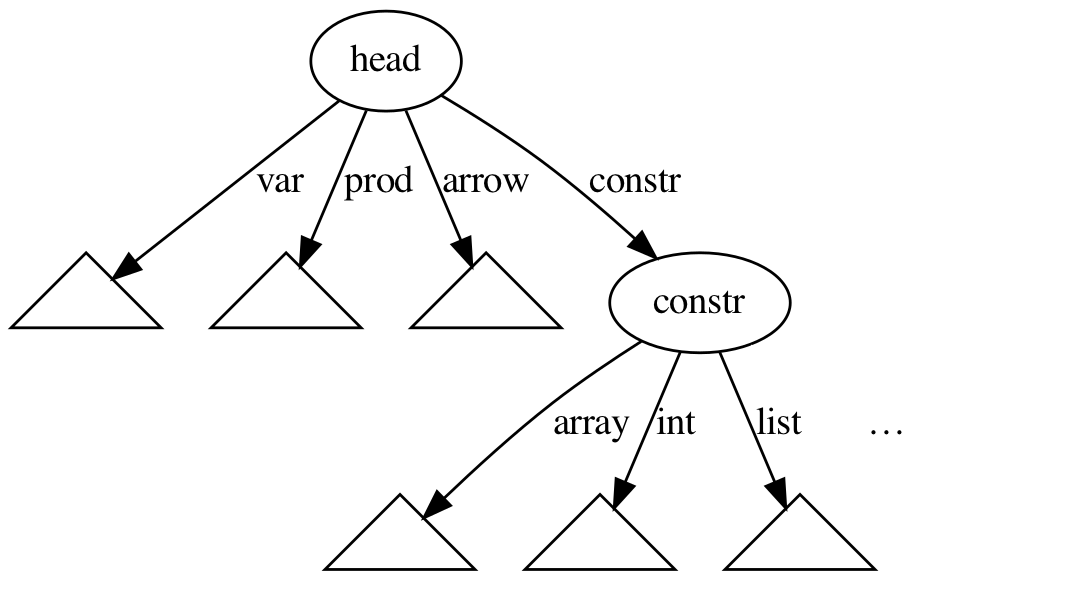
\includegraphics[scale=0.2]{graphs/by_head}
\end{center}
\end{figure}

TODO

%============================================================

\subsection{Deuxième critère}

TODO

%============================================================
%============================================================

\section{Structure de \trie}

\begin{figure}[h]
\begin{center}
	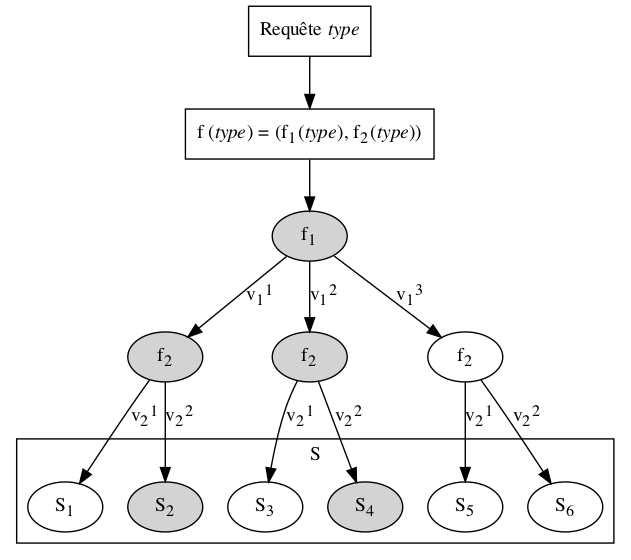
\includegraphics[scale=0.3]{graphs/trie}
\end{center}
\end{figure}

\begin{minted}{ocaml}
module type FEATURE = sig
  type t
  val compute : Type.t -> t
  val compare : t -> t -> Int.t
  val compatible : query:t -> data:t -> Bool.t
end
\end{minted}

\begin{minted}{ocaml}
module type NODE = sig
  type t
  val empty : t
  val add : Type.t -> t -> t
  val remove : Type.t -> t -> t
  val iter : t -> Type.t Iter.t
  val iter_with : Type.t -> t -> Type.t Iter.t
end

module Leaf : NODE
module Node (Feat : FEATURE) (Sub : NODE) : NODE
\end{minted}

TODO
\begin{itemize}
	\item motivation avec \cite{Schulz}
	\item interface OCaml : Feature, Trie
	\item exemples
\end{itemize}

%============================================================
%============================================================
%============================================================

\chapter{\dowsindex}

TODO
\begin{itemize}
	\item sélection de librairies
	\item incrémental
	\item matching
\end{itemize}

\begin{figure}[h]
\begin{center}
	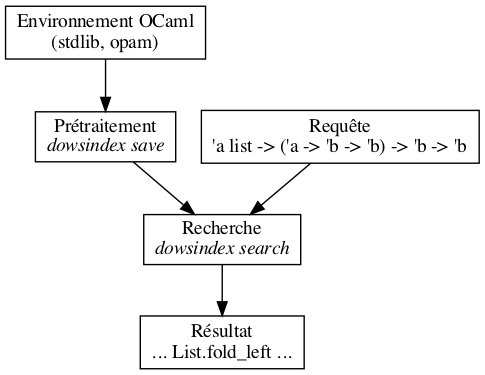
\includegraphics[scale=0.35]{graphs/dowsindex}
\end{center}
\end{figure}

%============================================================
%============================================================

\section{\dowsindex \texttt{save}}

La commande \dowsindex \texttt{save} admet les options suivantes :

\begin{table}[h]
\begin{tabular}{ll}
		\textbf{-{}-index}=\textit{fichier} &
		Sauvegarde l'index dans \textit{fichier}. \\ &
		Par défaut : dans un répertoire standard propre à stocker les données d'applications.
	\\
		\textbf{-{}-verbose} &
		Active le mode verbeux. Affiche les paquets trouvés.
\end{tabular}
\end{table}

TODO
\begin{itemize}
	\item présentation
	\item exemples : varier nombre de paquets, mise à jour
\end{itemize}

%============================================================
%============================================================

\section{\dowsindex \texttt{stats}}

La commande \dowsindex \texttt{stats} admet les options suivantes :

\begin{table}[h]
\begin{tabular}{ll}
		\textbf{-{}-filter} &
		Calcule aussi les statistiques avec filtrage par critères.
	\\
		\textbf{-{}-index}=\textit{fichier} &
		Cherche l'index dans \textit{fichier}. \\ &
		Par défaut : dans un répertoire standard propre à stocker les données d'applications.
	\\
		\textbf{-{}-measure}=\textit{mesure} &
		Mesure les types avec \textit{mesure}.
\end{tabular}
\end{table}

TODO
\begin{itemize}
	\item présentation
	\item exemples
\end{itemize}

%============================================================
%============================================================

\section{\dowsindex \texttt{search}}

La commande \dowsindex \texttt{search} admet les options suivantes :

\begin{table}[h]
\begin{tabular}{ll}
		\textbf{-{}-exhaustive} &
		Recherche exhaustive (sans filtrage par critères).
	\\
		\textbf{-{}-index}=\textit{fichier} &
		Cherche l'index dans \textit{fichier}. \\ &
		Par défaut : dans un répertoire standard propre à stocker les données d'applications.
	\\
		\textbf{-n} \textit{n} &
		Affiche les \textit{n} premiers résultats seulement.
\end{tabular}
\end{table}

TODO
\begin{itemize}
	\item présentation
	\item exemples : varier nombre de paquets, types plus ou moins complexes
\end{itemize}

%============================================================
%============================================================

\section{Extensions}

\begin{figure}[h]
\begin{center}
	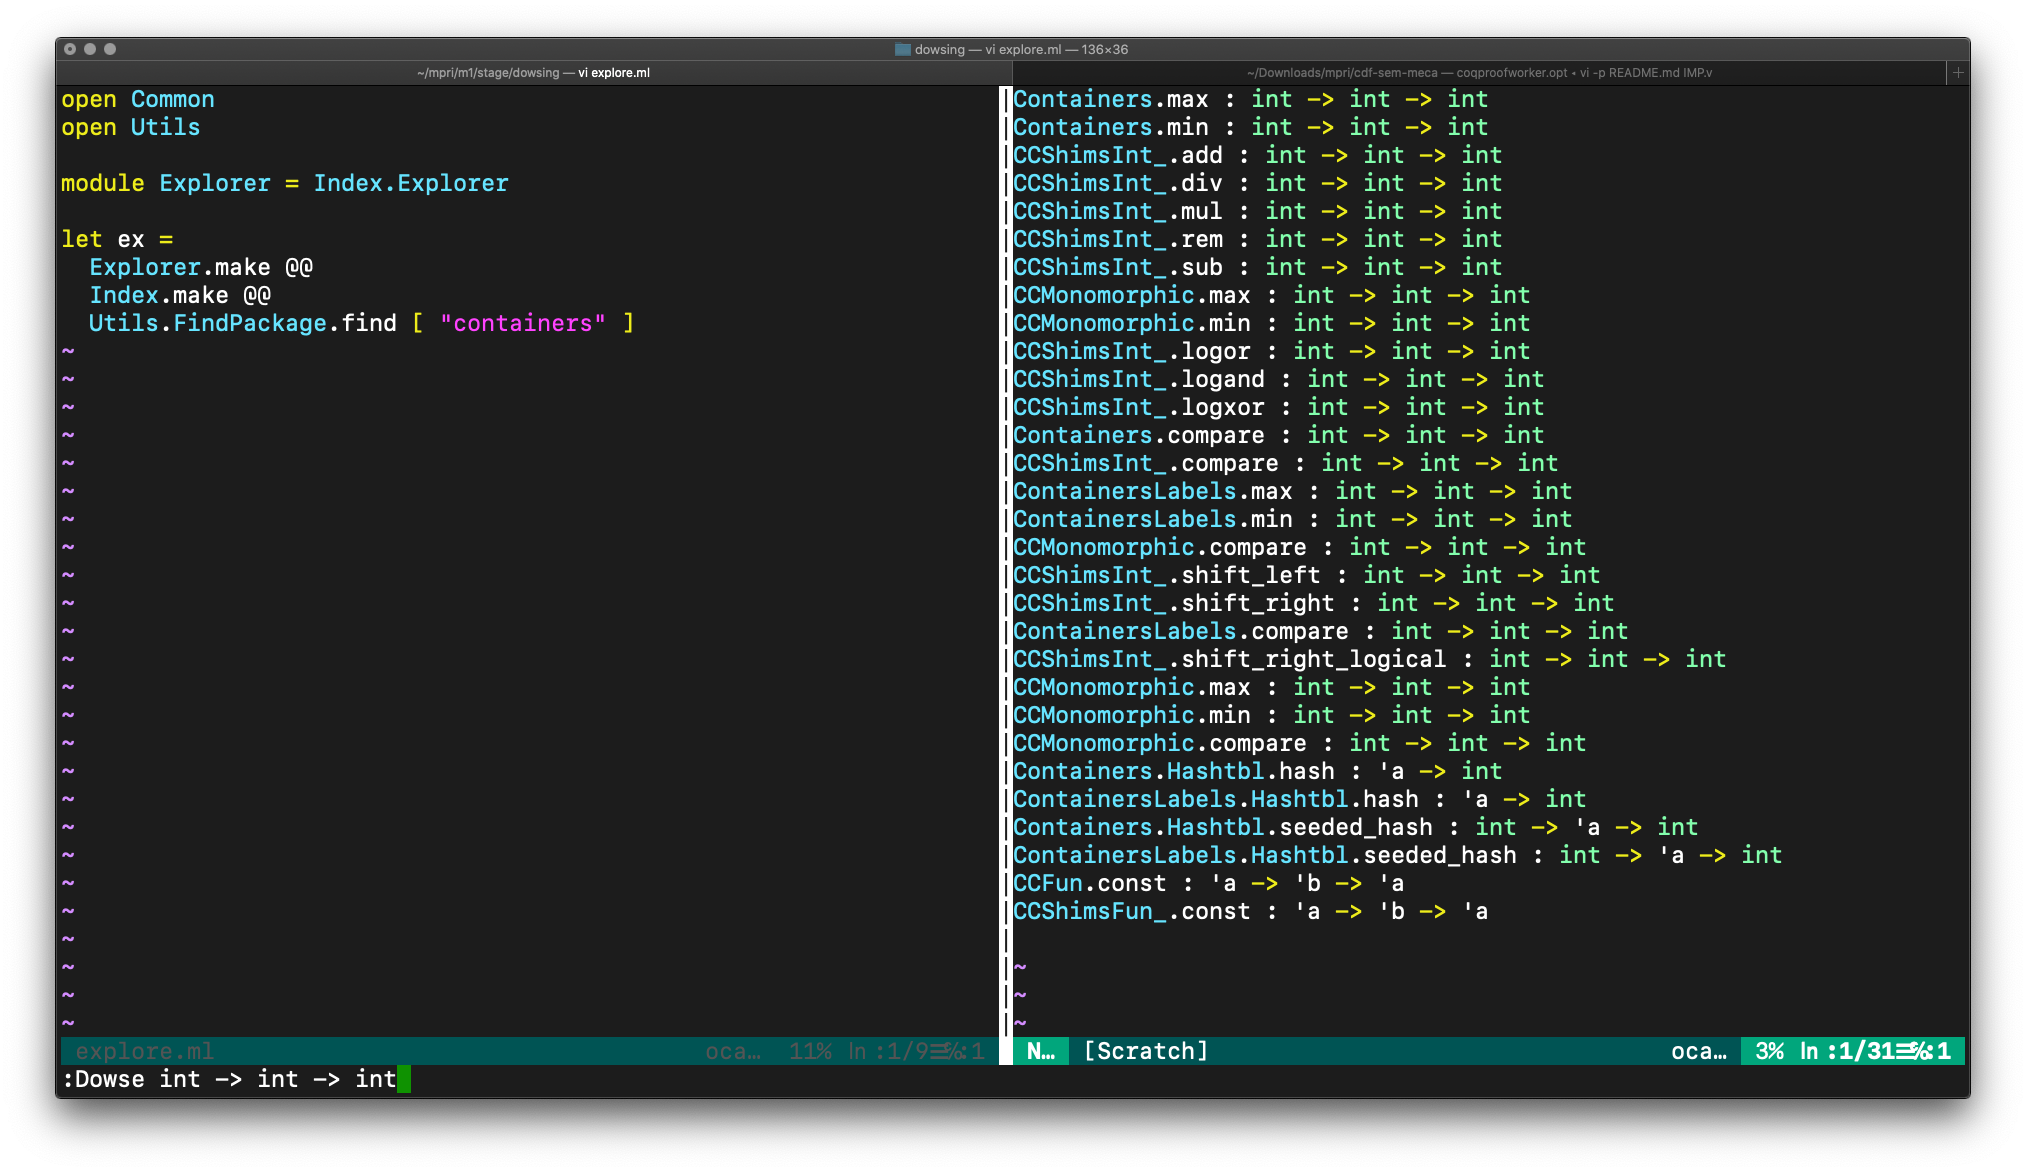
\includegraphics[scale=0.15]{images/vim_plugin}
\end{center}
\end{figure}

TODO

%============================================================
%============================================================
%============================================================

\chapter{Conclusion}

TODO
\begin{itemize}
	\item problèmes noms : qualification par rapport au module englobant
	\item alias de type
	\item temps de construction de l'index (LibIndex)
	\item temps de chargement de l'index (Marshall)
\end{itemize}

%============================================================
%============================================================
%============================================================

\chapter* {Annexe}
\addcontentsline{toc}{chapter}{Annexe}

Cette annexe est dévolue à la démonstration des conditions nécessaires d'unifiabilité sans l'axiome ($*$-unit). Son inclusion complexifie considérablement le travail ; nous n'en sommes pas encore venus à bout.

%============================================================
%============================================================

\section{Premier critère}

\begin{definition}[racine d'un type]
	La racine d'un type, notée $[ \cdot ]$, est le symbole défini inductivement par :
	\begin{align*}
			[ \alpha ] &= \alpha
		\\
			[ \unit ] &= \unit
		\\
			[ \tau_1 \times \tau_2 ] &= \times
		\\
			[ \tau_1 \rightarrow \tau_2 ] &=\ \rightarrow
		\\
			[ f (\tau_1, \dots, \tau_{|f|_\F}) ] &= f
	\end{align*}
\end{definition}

\begin{lemme} \label{equiv_tete}
	Si deux types sont équivalents, leurs têtes le sont aussi.
\end{lemme}

\begin{lemme} \label{tete_subst_tete}
	\[ \forall \tau \in T,\ \forall \sigma \in \Sigma,\ \uparrow \hat \sigma (\tau) =\ \uparrow \hat \sigma (\uparrow \tau) \]
\end{lemme}

\begin{lemme} \label{tete_non_fleche}
	La tête d'un type n'est pas une flèche.
\end{lemme}

\begin{lemme} \label{cons_equiv}
	\[
		\forall f_1 \in \F ,\ 
		\forall f_2 \in \F,\ 
		\forall (\tau^1_i)_{i \in \interval 1 {|f_1|_\F}} \in T^{|f_1|_\F},\ 
		\forall (\tau^2_i)_{i \in \interval 1 {|f_2|_\F}} \in T^{|f_2|_\F},
	\]\[
		f_1 (\tau^1_1, \dots, \tau^1_{|f_1|_\F}) =
		f_2 (\tau^2_1, \dots, \tau^2_{|f_2|_\F})
		\implies f_1 = f_2
	\]
\end{lemme}

\begin{theoreme}
	Si deux types $\tau_1$ et $\tau_2$ sont unifiables et les racines de leurs têtes appartiennent à $\F$, alors ces racines sont les mêmes.
\end{theoreme}

\begin{preuve}
	Par hypothèse, il existe une substitution $\sigma$ telle que :
	\[ \hat \sigma (\tau_1) \Tequiv \hat \sigma (\tau_2) \]
	Par le lemme \ref{equiv_tete}, les têtes sont équivalentes :
	\[ \uparrow \hat \sigma (\tau_1) \Tequiv\ \uparrow \hat \sigma (\tau_2) \]
	Par le lemme \ref{tete_subst_tete}, on a donc :
	\[ \uparrow \hat \sigma (\uparrow \tau_1) \Tequiv\ \uparrow \hat \sigma (\uparrow \tau_2) \]
	Par hypothèse, il existe $f_1$ et $f_2$ dans $\F$ ainsi que $(\tau^1_i)_{i \in \interval 1 {|f_1|_\F}}$ dans $T^{|f_1|_\F}$ et $(\tau^2_i)_{i \in \interval 1 {|f_2|_\F}}$ dans $T^{|f_2|_\F}$ tels que :
	\begin{align*}
			\tau_1 &= f_1 (\tau^1_1, \dots \tau^1_{|f_1|_\F})
		\\
			\tau_2 &= f_2 (\tau^2_1, \dots \tau^2_{|f_2|_\F})
	\end{align*}
	Par le lemme \ref{tete_non_fleche}, $f_1$ et $f_2$ sont différents de $\rightarrow$. Par definition de $\uparrow \cdot$ et $\hat \sigma$, il vient alors :
	\[ f_1 (\hat \sigma (\tau^1_1), \dots, \hat \sigma (\tau^1_{|f_1|_\F})) \Tequiv f_2 (\hat \sigma (\tau^2_1), \dots, \hat \sigma (\tau^2_{|f_2|_\F})) \]
	Enfin, le lemme \ref{cons_equiv} donne :
	\[ f_1 = f_2 \]
\end{preuve}

%============================================================
%============================================================

\section{Deuxième critère}

\begin {definition} [multiplicité d'un symbole de fonctions]
	La multiplicité d'un symbole $f$ de $\F$ dans un type $\tau$, notée $\mu_f (\tau)$, est définie inductivement par :
	\begin{align*}
			\mu_f (\tau_1 \rightarrow \tau_2) &=
			\mu_f' (\tau_1) + \mu_f (\tau_2)
		\\
			\mu_f (\tau) &=
			0
		\\
			\mu_f' (\tau_1 \times \tau_2) &=
			\mu_f' (\tau_1) + \mu_f' (\tau_2)
		\\
			\mu_f' (f (\tau_1, \dots, \tau_n)) &=
			1
		\\
			\mu_f' (\tau) &=
			0
	\end{align*}
\end{definition}

\begin{definition}[$\V$-multiplicité]
	La $\V$-multiplicité est définie inductivement par :
	\begin{align*}
			\mu_\V (\tau_1 \rightarrow \tau_2) &=
			\mu_\V' (\tau_1) + \mu_\V (\tau_2)
		\\
			\mu_\V (\tau) &=
			0
		\\
			\mu_\V' (v) &=
			1
		\\
			\mu_\V' (\tau_1 \times \tau_2) &=
			\mu_\V' (\tau_1) + \mu_\V' (\tau_2)
		\\
			\mu_\V' (\tau) &=
			0
	\end{align*}
\end{definition}

\begin{definition}[type simple]
	Un type $\tau$ est simple si sa $\V$-multiplicité est nulle.
\end{definition}

\begin{lemme} \label{mu_equiv}
	Si deux type $\tau_1$ et $\tau_2$ sont équivalents, alors, pour tout symbole $f$ de $\F$, on a : $\mu_f (\tau_1) = \mu_f (\tau_2)$.
\end{lemme}

\begin{lemme} \label{mu_subst_simple}
	Si un type $\tau$ est simple, alors, pour tout symbole $f$ de $\F$ et toute substitution $\sigma$, on a : $\mu_f (\hat \sigma (\tau)) = \mu_f (\tau)$.
\end{lemme}

\begin{lemme} \label{mu_subst}
	La multiplicité de tout symbole $f$ de $\F$ dans un type est inférieure à celle de toute instance de ce type.
\end{lemme}

\begin{theoreme}
	Soit deux types $\tau_1$ et $\tau_2$. \\
	Si $\tau_1$ et $\tau_2$ sont unifiables et $\tau_1$ simple, alors la multiplicité de tout symbole de $\F$ dans $\tau_1$ est supérieure à celle dans $\tau_2$.
\end{theoreme}

\begin{preuve}
	Par hypothèse, il existe une substitution $\sigma$ telle que :
	\[ \hat \sigma (\tau_1) \Tequiv \hat \sigma (\tau_2) \]
	Soit $f$ un symbole de $\F$. Par le lemme \ref{mu_equiv}, les multiplicités sont égales :
	\[ \mu_f (\hat \sigma (\tau_1)) = \mu_f (\hat \sigma (\tau_2)) \]
	Par le lemme \ref{mu_subst_simple}, la simplicité de $\tau_1$ apporte :
	\[ \mu_f (\hat \sigma (\tau_1)) = \mu_f (\tau_1) \]
	Par le lemme \ref{mu_subst}, on a par ailleurs :
	\[ \mu_f (\hat \sigma (\tau_2)) \geqslant \mu_f (\tau_2) \]
	Il vient donc le résultat attendu :
	\[ \mu_f (\tau_1) \geqslant \mu_f (\tau_2) \]
\end{preuve}

%============================================================
%============================================================
%============================================================

\printbibliography

\end{document}


























%%% Local Variables:
%%% mode: latex
%%% TeX-master: t
%%% TeX-command-extra-options: "-shell-escape"
%%% End:
